
\documentclass[a4paper,10pt]{article}
%\usepackage{fullpage}
\usepackage[swedish]{babel}
\usepackage{todonotes}

\usepackage{url}
\usepackage{titlesec}

%\usepackage{algorithmicx}
\usepackage{algorithm}
\usepackage{algpseudocode}
\algnewcommand{\LineComment}[1]{\State \(\triangleright\) #1}
\algnewcommand{\Continue}{\textbf{continue}}
\algnewcommand{\Vspace}{\item[]}
\algnewcommand{\To}{\textbf{to}~}

\usepackage{mathtools}
\DeclarePairedDelimiter\ceil{\lceil}{\rceil}
\DeclarePairedDelimiter\floor{\lfloor}{\rfloor}
\newcommand{\addeq}{\mathrel{+}=}
\newcommand{\subeq}{\mathrel{-}=}
\newcommand{\unioneq}{\mathrel{\cup}=}
\newcommand{\addadd}{\mathrel{++}}
\newcommand{\subsub}{\mathrel{--}}

\usepackage{framed}

%\usepackage[section]{placeins}

\usepackage{graphicx}
\usepackage{caption}
\usepackage{subcaption}

\usepackage{amsmath}

\title{Digitally transmitting a sound signal over RF radio}

\author{Bj{\"o}rn Forsberg \and Sven Lundgren \and Jonathan Sharyari}
%\textwidth 5.5in 
%\oddsidemargin 0.5in 

\begin{document}

\maketitle

\section{Sammanfattning}

Denna rapport beskriver en implementation av ett system för digital 
ljudöverföring som en del av projektdelen i kursen Digitalteknik och Elektronik 
(1TE717). Systemet använder en mikrofon för att ta upp ljudvågor, vilka sedan
konverteras till en digital signal och sänds via radio till en mottagare.
Mottagaren konverterar tillbaka signalen till den analoga representationen som
sedan kan spelas upp på en högtalare. Den digitala överföringen minskar risken
för störningar i överföringen, då risken att en etta och nolla ska flippa är 
mindre än risken för störningar på en analog signal.

Vid enklare tester visar sig systemet kapabelt att föra över mycket exakta 
signaler från sändare till mottagare. Det är dock mycket känsligt för att hamna
i otakt, i det att överföringen inte har någon tydlig början och slut. I och med
detta måste mottagaren manuellt synkronisera signalen. Detta måste dock endast
göras en gång vid systemstart. Slutligen använder denna implementation en delad
klocksignal mellan sändare och mottagare, vilket reducerar den praktiska 
användbarheten av systemet. Det lämnas till framtida arbete att implementera en
distribuerad klockning av systemet.


\section{Inledning}

Att överföra ljud elektroniskt mellan två punkter är ett av de största 
genombrotten inom kommunikation. Det har tillåtit vänner och familjer  att hålla 
kontakten över stora avstånd, gjort det möjligt för stater att kommunicera i i
stort sett realtid.

Traditionellt sett har ljudsignalerna överförts från vibrationer i luften till
förändringar i elektrisk spänning med hjälp av en mikrofon. I denna analoga 
representation, motsvaras tryckförändringar i luften direkt av 
spänningsförändringar i mikrofonens utsignal. På motsvarande sätt överförs de
elektriska signalerna tillbaka till ljudsignaler via en högtalare, genom att 
framkalla tryckförändringar i luften motsvarande spänningsförändringarna i
den elektriska signalen.

I dag sker allt större delar av världens informationsöverföring i digital form, 
där informationen istället uttrycks i sekvenser av höga (t.ex. $5V$) och låga
(t.ex. $0V$) signaler. För att representera ljudvågor digitalt behöver således 
tryckförändringarna i luften översättas till diskreta värden, som kan 
representeras av ett tal.
Exempelvis kan intervallet $[u^{min}, u^{max}]$ delas upp i $n$ diskreta 
delintervall, var och en representerad av ett binärt tal. Ju högre man väljer
$n$, desto fler bitar behövs för att representera alla delintervall. Antalet 
intervall som kan representeras ges av uttrycket $n = 2^b$ där $b$ är antalet 
bitar som används för att uttrycka värdet. Elektriska komponenter som översätter
analoga spänningar till dess digitala representation kallas 
analog-till-digital-omvandlare (AD-omvandlare, ADC). 
För att återföra den digitala signalen till sin analoga form används en
digital-till-analog-omvandlare (DA-omvandlare, DAC), och dess funktion är
inversen av ADC:ns. 

Denna rapport presenterar ett projekt om $4 hp$, i vilket ett 
ljudöverföringssystem presenteras. Med hjälp av en mikrofon fångas en 
ljudsignal upp, omvandlas till en digital representation, varpå denna digitala 
representation överförs seriellt via radiovågor till en mottagare. Mottagaren i 
sin tur omvandlar den digitala representationen tillbaka till en analog signal 
som kan omvandlas till ljud av en högtalare.

Att gå igenom dessa steg för att omvandla en analog signal till en digital, för
att sedan direkt återföra den till den analoga representationen kan låta 
onödigt, men motiveras utav den lägre störningsrisken i digital överföring. 
Detta eftersom att en störning på en analog signal överlagras in i signalen, och
det är kostsamt att rensa ut dessa störningar. I motsats kommer en störning på
en digital signal i normalfallet inte påverka informationen i signalen, eftersom
att störningen måste vara mycket stor för att signalens betydelse ska skifta
mellan logiskt hög och låg.


\section{Genomförande}

Implementeringen av kretsen gjordes med ett enkelt kombinatoriskt nät som ger
styrsignalerna till ADC och DAC. Ut- respektive insignalerna till ADC och DAC
förs sedan över via radio. De komponenter som använts presenteras i Tabell 
\ref{tab:komponenter}. Resterande del av denna sektion är uppdelat i fyra
undersektioner, den första beskriver implementationen av mikrofonkretsen, den 
varefter den andra beskriver implementationen av sändaren, och slutligen den 
tredje beskriver implementationen av mottagaren. För att spela upp
utsignalen användes en färdig högtalare inbyggd i kopplingsborden som användes,
och därför beskrivs denna komponent ej närmre. Slutligen beskrivs hur de 
synkrona komponenterna i systemet klockas.

\begin{table}
    \centering
    \begin{tabular}{|l|l|}
    \hline
    1 st & Texas Instruments ADS7816P, 12-bit ADC, DIP-8 \\
    1 st & Texas Instruments DAC7611P, 12-bit DAC, DIP-8 \\
    1 st & Mikrofon \\
    2 st & TODO Räknare \\
    2 st & TODO 4-AND \\
    1 st & TODO 2-XOR \\
    1 st & TODO NOT \\
	 & Funktionsgenerator \\
    \hline
    \end{tabular}
    
    \caption{Komponenterna som använts för att implementera .}
    \label{tab:komponenter}

\end{table}

\subsection{Mikrofon}



\subsection{Sändare}

Den mest centrala komponenten i sändaren är ADC:n, som konverterar den analoga
signalen från mikrofonen till en 12-bitars digital signal som sedan sänds över
radio.

Det finns ett mycket stort utbud av integrerade kretsar för ADC:er på marknaden,
med flera inbördes olika egenskaper. Det första att ta hänsyn till vid valet av
ADC är seriell eller parallel utsignal. Eftersom att utsignalen skickas över 
radio som en seriell signal är valet av seriell ADC uppenbart. För seriella 
komponenter finns sedan åtskilliga val vad gäller protokoll som kontrollerar när
och hur data skickas ut från komponenten. I detta fall föll valet på en 
SPI-bestyckad ADC, eftersom att SPI är ett förhållandevis enkelt protokoll, och
därmed lätt att kontrollera med hjälp av enkla kombinatoriska nät, i motsats 
till mer avancerade protokoll där en mikrokontroller är mer eller mindre
nödvändig. Eftersom att SPI definerar hur data förs över rent fysiskt mycket
hårdare än det definerar vilken data som skickas, finns det flera olika 
implementationer av dataprotokollet. Det slutgiltiga valet föll på $ADS7816P$,
en SPI-bestyckad 12-bitars ACD med ett mycket enkelt dataprotokoll, vilken 
därför kräver ett mycket enkelt kombinatoriskt när för att styra.

\todo{skriv mer när ålands bilder finns}



\subsection{Mottagare}

Liksom för sändaren är det konverteringen mellan analog och digital data som
är den centrala funktionen i mottagaren. I detta fall är det den digitala 
signalen som mottages över radio som ska konverteras tillbaka till en analog
signal som kan tolkas av högtalaren.

Liksom för valet av ADC i sändaren finns det en stor variation av tillgängliga 
DAC:ar på marknaden. Eftersom att mottagaren ska vara kompatibel med sändaren
är även denna 12-bitars seriell, och liksom ADC:n föll protokollvalet på SPI. 
Även här var en enkel implementation av SPI avgörande och därför valdes 
slutligen $DAC7611P$ för mottagarens DA-omvandling. 

Denna DAC kräver förutom $CS$-signalen även en $LD$-signal för att ladda in data
i registret. Detta ger ett något mer komplicerat grindnät än på sändarsidan, och
3 grindar krävs för att producera de tre insignalerna.


\begin{figure}
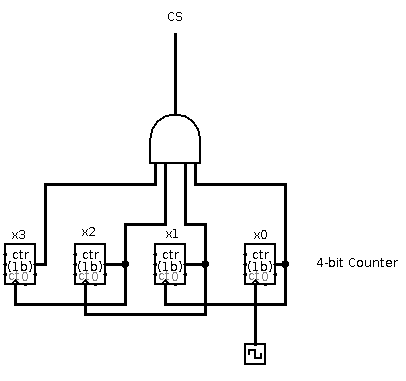
\includegraphics{adccircuit.png}
\caption{bsadfsafs}
\label{adccircuit}
\end{figure}
\begin{figure}
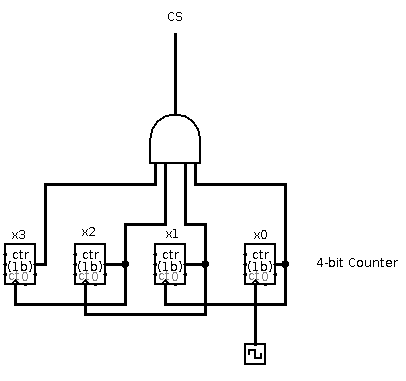
\includegraphics{adccircuit.png}
\caption{bsadfsafs}
\label{adccircuit}
\end{figure}
\begin{figure}
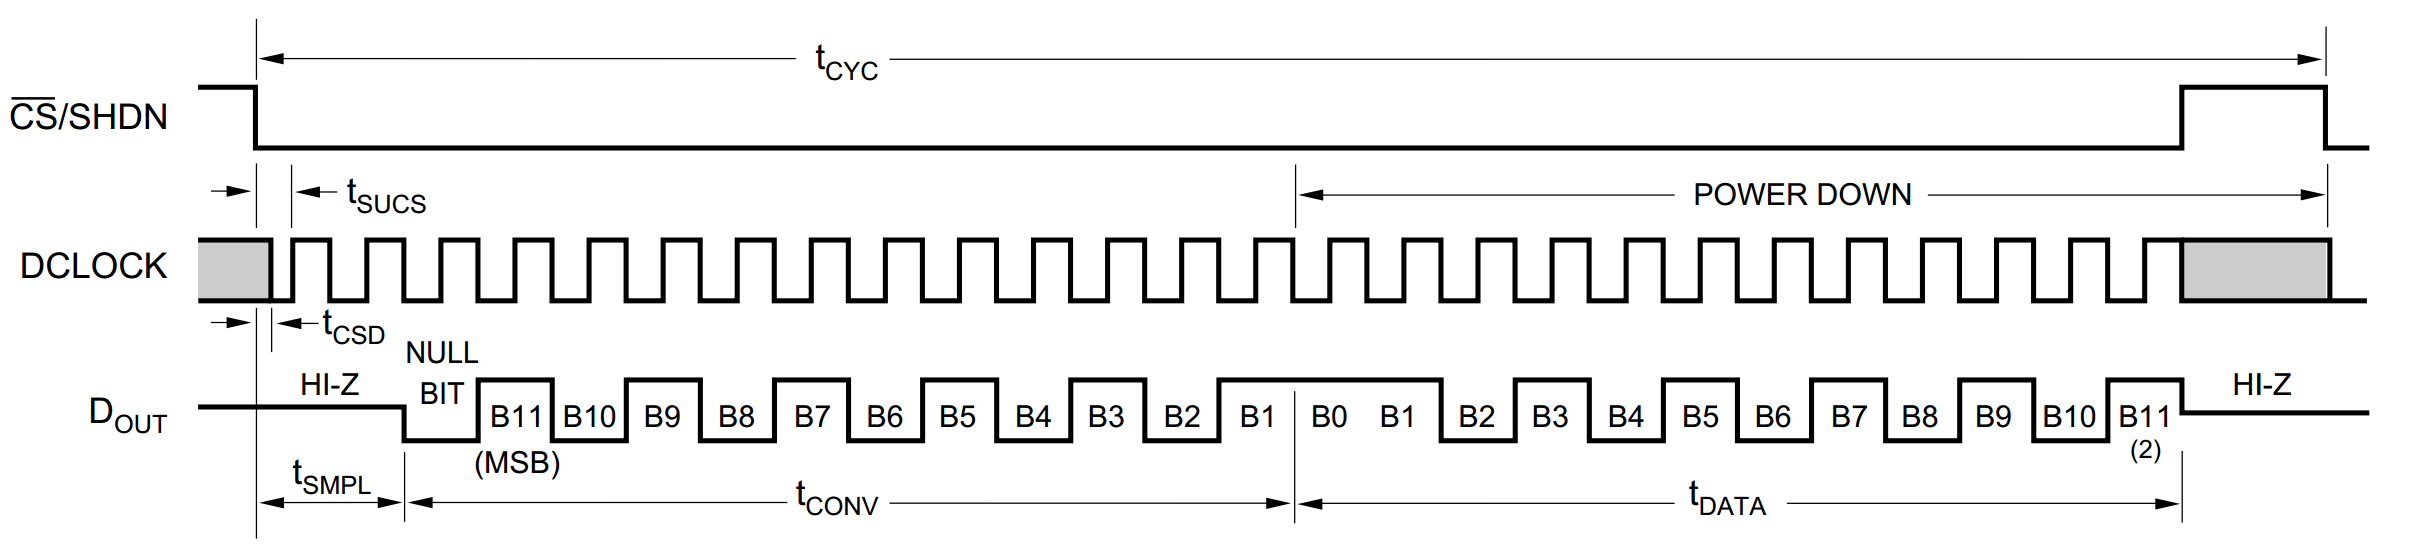
\includegraphics{adcdiagram.png}
\caption{bsadfsafs}
\label{adccircuit}
\end{figure}
\begin{figure}
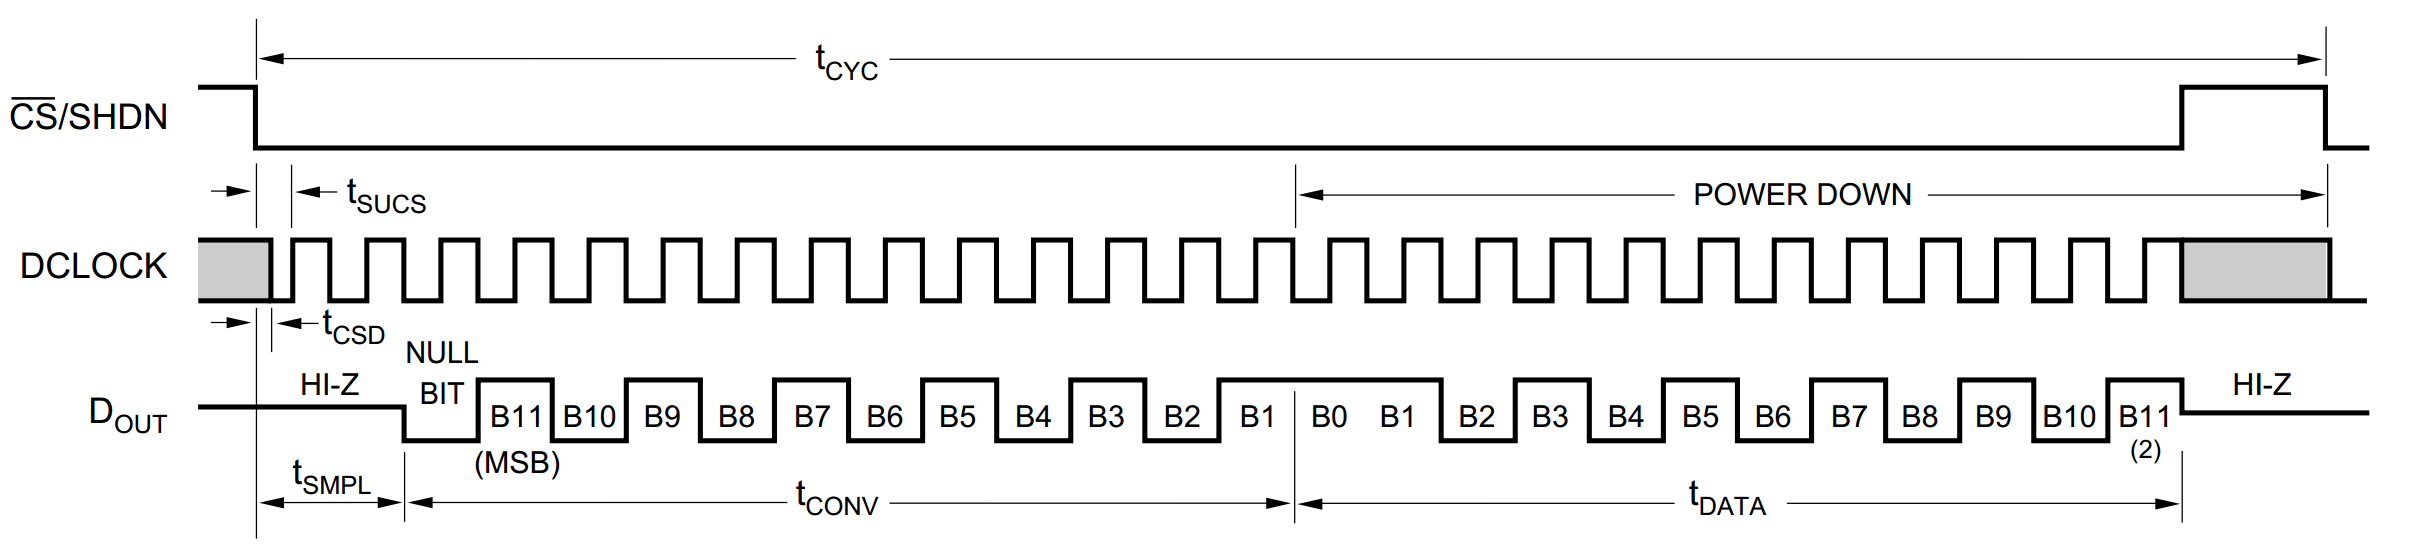
\includegraphics{adcdiagram.png}
\caption{bsadfsafs}
\label{adccircuit}
\end{figure}

\begin{tabular}{c c c c| c c}
$x_3$ & $x_2$ & $x_1$ & $x_0$ & $cs$ & $ld$ \\\hline
0 & 0 & 0 & 0 & 0 & 1 \\
0 & 0 & 0 & 1 & 0 & 1 \\
0 & 0 & 1 & 0 & 0 & 1 \\
0 & 0 & 1 & 1 & 0 & 1 \\
0 & 1 & 0 & 0 & 0 & 1 \\
0 & 1 & 0 & 1 & 0 & 1 \\
0 & 1 & 1 & 0 & 0 & 1 \\
0 & 1 & 1 & 1 & 0 & 1 \\
1 & 0 & 0 & 0 & 0 & 1 \\
1 & 0 & 0 & 1 & 0 & 1 \\
1 & 0 & 1 & 0 & 0 & 1 \\
1 & 0 & 1 & 1 & 0 & 1 \\
1 & 1 & 0 & 0 & 1 & 1 \\
1 & 1 & 0 & 1 & 1 & 0 \\
1 & 1 & 1 & 0 & 1 & 0 \\
1 & 1 & 1 & 1 & 1 & 1 \\
\end{tabular}

$cs$ = $x_3 \wedge x_2$
$ld$ = $x3 \wedge x_2 \wedge (x_1 \oplus x_0)$


\begin{tabular}{c c c c| c}
$x_3$ & $x_2$ & $x_1$ & $x_0$ & $cs$ \\\hline
0 & 0 & 0 & 0 & 0 \\
0 & 0 & 0 & 1 & 0 \\
0 & 0 & 1 & 0 & 0 \\
0 & 0 & 1 & 1 & 0 \\
0 & 1 & 0 & 0 & 0 \\
0 & 1 & 0 & 1 & 0 \\
0 & 1 & 1 & 0 & 0 \\
0 & 1 & 1 & 1 & 0 \\
1 & 0 & 0 & 0 & 0 \\
1 & 0 & 0 & 1 & 0 \\
1 & 0 & 1 & 0 & 0 \\
1 & 0 & 1 & 1 & 0 \\
1 & 1 & 0 & 0 & 0 \\
1 & 1 & 0 & 1 & 0 \\
1 & 1 & 1 & 0 & 0 \\
1 & 1 & 1 & 1 & 1 \\
\end{tabular}

$cs$ = $x_3 \wedge x_2 \wedge x_1 \wedge x_0$

\subsection{Klocka och klockpulser}

Systemet använder sig av flera synkrona integrerade kretsar som kräver en
klockpuls. Digitalisering av tal kräver att ljudsignalen samplas i minst 
\todo*{XX} Hz för att fånga upp alla nyanser av ljudsignalen. Detta innebär att 
en snabb klockpuls måste ges till hela systemet, vilket i sin tur kräver 
komponenter som tål denna höga klockpuls. Utöver DAC och ADC är det räknaren som 
kontrollerar styrsignalerna till dessa, som är beroende av klockpulsen. 

Eftersom att klocksynkronisering är ett stort och välkänt problem, har det 
utelämnats i detta projekt, och klockpulsen delas således av sändare och 
mottagare i den nuvarande implementationen. En implementation av en distribuerad 
klocka skulle därför innebära ett eget projekt i sig. Detta innebär att även om 
data överförs trådlöst är systemet fortfarande beroende av en delad kabel. 

\todo{finns nog rätt mycket mer att skriva}

\section{Resultat}

Det implementerade systemet klarar av att störningsfritt överföra ljudsignaler
mellan sändaren och mottagaren. 

\section{Diskussion}

\section{Bibliografi}

\begin{thebibliography}{hejhej}

\end{thebibliography}


\end{document}
